% プロジェクト学習中間報告書書式テンプレート ver.1.0 (iso-2022-jp)

% 両面印刷する場合は `openany' を削除する
\documentclass[openany,11pt,papersize]{jsbook}

% 報告書提出用スタイルファイル
\usepackage[final]{funpro}%最終報告書
%\usepackage[middle]{funpro}%中間報告書

% 画像ファイル (EPS, EPDF, PNG) を読み込むために
\usepackage[dvipdfmx]{graphicx,color}

% ここから -->
\usepackage{calc,ifthen}
\newcounter{hoge}
\newcommand{\fake}[1]{\whiledo{\thehoge<70}{#1\stepcounter{hoge}}%
  \setcounter{hoge}{0}}
% <-- ここまで 削除してもよい

\usepackage{here}

% 年度の指定
\thisYear{2015}

% プロジェクト名
\jProjectName{フィールドから創る地域・社会のためのスウィフトなアプリ開発}

% [簡易版のプロジェクト名]{正式なプロジェクト名}
% 欧文のプロジェクト名が極端に長い(2行を超える)場合は、短い記述を
% 任意引数として渡す。
%\eProjectName[Making Delicious curry]{How to make delicious curry of Hakodate}
\eProjectName{“Swift” Application Development Based on Field Research}


% <プロジェクト番号>-<グループ名>
\ProjectNumber{3-C}

% グループ名
\jGroupName{教育系グループ}
\eGroupName{Education Group}

% プロジェクトリーダ
\ProjectLeader{1013220}{新保遥平}{Yohei~Shinpo}

% グループリーダ
\GroupLeader  {1013015}{中進吾}{Shingo~Naka}

% メンバー数
\SumOfMembers{5}
% グループメンバ
\GroupMember  {1}{1013130}{熊谷優斗}{Yuto~Kumagai}
\GroupMember  {2}{1013116}{皀勢也}{Seiya~Kurokome}
\GroupMember  {3}{1013220}{新保遥平}{Yohei~Shinpo}
\GroupMember  {4}{1013015}{中進吾}{Shingo~Naka}
\GroupMember  {5}{1013104}{矢吹渓悟}{Keigo~Yabuki}

% 指導教員
\jadvisor{伊藤恵,奥野拓,原田泰,木塚あゆみ,南部美砂子}
% 複数人数いる場合はカンマ(,)で区切る。カンマの前後に空白は入れない。
\eadvisor{Kei~Itou,Taku~Okuno,Yasushi~Harada,Ayumi~Kizuka,Misako~Nanbu}

% 論文提出日
\jdate{2015年7月29日}
\edate{July~29, 2015}

%%%%%%%%%%%%%%%%%%%%%%%%%%%%%%%%%%%%%%%
\usepackage{graphicx}
%%%%%%%%%%%%%%%%%%%%%%%%%%%%%%%%%%%%%%%
\begin{document}
%
% 表紙
\maketitle

%前付け
\frontmatter

% 和文概要
\begin{jabstract} 
%\fake{ここに日本語の概要を書きます。}
 本プロジェクトは教育というフィールドを調査し、教育に関する問題を解決するiOSアプリを開発することを目的としている。

 プロジェクトの当初は、各メンバーが教育に関わるアプリを考え、メンバーと担当教員にプレゼンテーションを行った。メンバー間では情報の共有を行い、担当教員からはレビューを受けた。その後、担当教員から受けたレビューを基に、お互いにアイデアを広げテーマを1つに絞り込んだ。テーマは、大学生向けプログラミング入門アプリに決まった。

 テーマが決まった後、アプリの設計を行った。しかし、要件定義を固めずにアプリの設計を行ったため、一貫性のないアプリ設計になってしまった。そのため、要件定義を1から考え直すことになった。要件定義を考え直すことは、1度で終わらず何度も行った。その結果、中学校でプログラミングを学んだ人、興味を持った人を対象にしたゲームアプリというテーマに決まった。

 中間発表では、私たちが考えた提案をポスターにまとめ、ポスターセッションを行った。教員や他学生からの評価シートには、「最終的なゴールは?」、「まだ内容が決まっていないので評価不能」、「既存のもとの比較がない」などの意見をいただき、もう1度要件定義を見直しアプリの設計をやり直す必要があることに気付かされた。

 今後は、アプリの設計をやり直しアプリを実装していくことを考えている。また、11月に開催されるアカデミックリンクにてワークショップを開き、そこで得たレビューをもとにアプリを改善していくことを考えている。

% 和文キーワード
%\begin{jkeyword}
%キーワード1, キーワード2, キーワード3, キーワード4, キーワード5
%\end{jkeyword}
\bunseki{中進吾}
\end{jabstract}

%英語の概要
\begin{eabstract} 
%\fake{you should write your English abstract in one page. }
 This project is having for its object to investigate a field as education and develop the iOS application useful for education.

 Each member considered the application of educating and presented a members and teachers on the first of a project. We shared information between the members and received reviews from teachers. After that ideas was expanded each other and the theme was narrowed down to 1 based on the review we received from teachers. The theme was decided in a programming guide application for college students.

 After the theme was decided, the application was designed. But the design of application had inconsistent because the application was designed without making the requirement definition hard. Therefore we changed the requirement definition from one. We didn't finish changing the requirement definition and went many times. As a result, it was decided in a theme as the game application that made the person who learned a programming at junior high school and an interested person the subject.

 The proposition that we thought was gathered in a poster and a poster session was performed in the middle announcement. We received opinions of which "what is last goal", "having no comparison it exists down", " the contents aren't decided yet, so evaluation is impossible" in an evaluation seat from teachers and other students, and the requirement definition was reconsidered again, and they made notice that it's necessary to redo a design of an application.

 We are thinking the design of application is being redone from now on and an application is being mounted. A workshop will be opened in the academic link held in November and we get the review and are thinking an application is being improved. 
% 英文キーワード
%\begin{ekeyword}
%Keyrods1, Keyword2, Keyword3, Keyword4, Keyword5
%\end{ekeyword}
\bunseki{中進吾}
\end{eabstract}

\tableofcontents% 目次


\mainmatter% 本文のはじまり

\chapter{背景}
\section{日本のプログラミング教育について}
日本では2012年から中学校の技術家庭科で、プログラミング教育が必修項目となっている。ビジュアルプログラミング言語のScratchやビュートビルダーなどを用いて授業を行っている。また、プログラミングを学ぶのは中学3年生の時だけである。

\bunseki{中進吾}

\section{現状と課題}
中学校ではビジュアル言語を用いた授業を行っており、ソースコードを書く練習はしていない。また、中学校でプログラミングを学べる期間は短い。そのため中学校の授業だけでは、ソースコードを書こうとした時、どのように組んでいいかわからない。
\bunseki{中進吾}

\chapter{本プロジェクトの目標}

\section{目的}\label{sec:mokuteki}
本プロジェクトの目的は、中学校でプログラミングを学んだ人、興味をもった人を対象として、中学で学んだプログラミングと実際のプログラミングの間のプロセスを支援し、ソースコードの組み立てを学ぶことが出来るゲームアプリを開発することである。
\bunseki{皀勢也}


\section{目標}
ビュートビルダーやScratchのようなビジュアルプログラミング言語を学んだ中学生が、C言語のように実際に文字を打ち込むようなソースコードの組み方を理解できるようになることが、本プロジェクトの目標である。
\bunseki{皀勢也}

%3章
\chapter{これまでの活動}

\section{プロジェクト全体としての活動}

\subsection{スクラッチワークショップへの参加}
\par 教育をテーマにするに当たり、まず小学生と触れ合い、教育の現状について考えるために、原田先生主催のワークショップに参加した。ワークショップは、2015年5月9日に、函館市青年センターにて行われ、小学校5年生から中学校1年生の子供達計10人が参加した。ワークショップの内容は、ビジュアルプログラミング言語「Scratch」を用いて、動きに反応して音が鳴る不思議楽器を作るというものである。当日、メンバーは小学生の側についてプログラミングのアシスタントをした。
\par ワークショップを通して、気づいた点は次の2点である。
\begin{itemize}
\item 子供達は、一度得た知識はすぐ自分のものにしているようだった。今回のワークショップは、前回のワークショップ参加者から引き続き参加している子供が多いということもあって、メンバーが使い方を教えるまでもなく、自力でプログラミングを行っていた。更に、繰り返し文の使い方を教えたところ、「じゃあさ、ここもこうすればいいんじゃない?」と、子供自ら別の点の修正を行っていた。子供の成長能力の高さに驚いた。
\item 前回から参加している子供に、どうして今回も参加したの?と尋ねたところ、「だって、これ(Scratch)楽しいんだもん」と答えた。子供でもプログラミングに興味を持っていることに驚いた。
\end{itemize}

\par また、ワークショップの最後に、参加者の子供達と、その親に向けた簡単なアンケートを実施した。しかし、プロジェクトとしての方針が決まってない状態で作成したアンケートだったため、内容が建設的なものではなく、得たアンケート結果をその後に生かすことが出来なかった。むしろ、アンケート内容に子供にはわかりづらい表現がある、難しい漢字を使っている、子供用と大人用のアンケート用紙の区別がつかないといった問題を発見できたことが、その後に生きる学びであったと言える。

\bunseki{熊谷優斗}

\subsection{リスク分析}
\par プロジェクトを進めるにあたって起こりうるリスクをメンバーそれぞれで洗い出し、それぞれのリスクに対して発生確率、被害の内容、対処方法を挙げた。図3.1は洗い出したリスクの一部である。

\par リスクの洗い出しをした時点で既に発生していたのが、「メンバーに連絡がつながらない」というリスクだ。前述のスクラッチワークショップにてアンケートを実施したが、このアンケートを作成する際、メンバーの1人に連絡がつながらず、ワークショップ当日になってそのメンバーにアンケート内容のレビューをしてもらった結果、いくつかの不備があることが発覚した。この不備は、そのメンバーが前日にアンケート内容をレビューできていれば気づけたはずである。今後このようなリスクが発生しないよう、メンバー内で1日1回はSkypeやLINEを確認することを義務づけた。

\begin{figure}[H]
\begin{center}
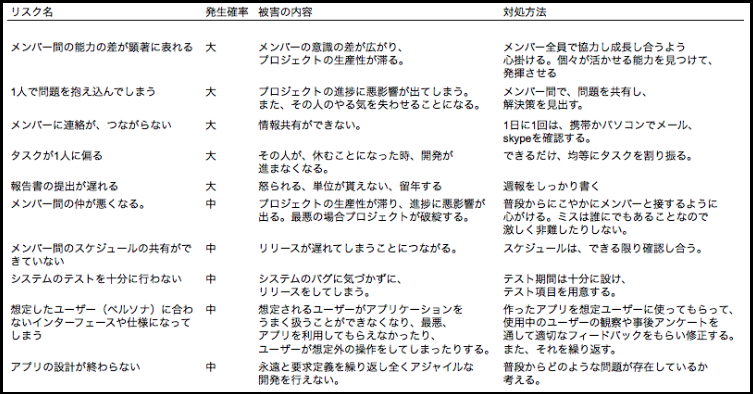
\includegraphics[width=14cm, bb=0 0 753 394]{img/RiskManagement.png}
\end{center}
\caption{リスク分析の結果(一部抜粋)}
\end{figure}

\bunseki{熊谷優斗}

\subsection{アプリ開発のための勉強会}
\par iOSアプリを開発するにあたって必要となる知識を学ぶ勉強会をプロジェクトのTAが開催したため、これにグループ全員で参加した。勉強会では、XcodeやSwift言語の使い方を学ぶSwift勉強会とバージョン管理システムである、GitとGitHubの使い方を学ぶGitHub勉強会の2種類が行われた。それぞれで行ったことを具体的に記述する。
\par Swift勉強会は全部で3回行われた。第1回では、メンバーそれぞれのPCにXcodeを導入し、Swift言語によってIBLabelやIBButtonを用いた簡単なアプリを作成した。その後、iPadにて作成したアプリをビルドするために、iOS Developer Programへの登録を行った。第2回では、MapKitというFrameworkを用いた地図アプリを作成した。第3回では、サーバーからデータを読み書きすることのできるアプリを作成した。それぞれの回の終わりには演習問題が出され、これを解くことで学んだ知識の復習を行うことができた。
\par GitHub勉強会は全部で3回行われた。それぞれの回を通して、バージョン管理システムの理念を学びつつ、Gitの基本的な使い方を学んでいった。第3回では、Swift勉強の演習問題をGitHubを用いてメンバー間で分担しながら作成せよ、という課題が出た。しかし、上手くコーディングの役割分担を行うことができず、1人で全てのコーディングをし、残りのメンバーでコードレビューをするという形を取った。これに対し、TAから昨年度はもっと役割分担ができていた、という報告を受けた。今後上手く役割分担をしていくために、教育班ではGitHubのissue機能を利用していくことを決定した。
\bunseki{熊谷優斗}

\subsection{バックログの作成}
\par プロジェクトの方針として、アジャイル開発手法の1つであるScrumという方法論を取り入れることに決まっていたため、プロジェクトのスケジュールをバックログを用いて管理した。バックログとは製品に必要な要素を項目に起こした一覧のことで、この一覧を上下に整頓することで項目の優先順位を表す。バックログには明確なスケジューリングをする必要はなく、優先順位の高いものから順番に行っていく。図3.2は6、7月分のバックログの原案である。

\par この原案を企業講師である高森満様と木下実様にお見せしたところ、「バックログの優先度を議論する際にもっと手軽に入れ替えることが可能なように、紙や付箋を用いたほうが良い」というレビューを受けた。そこで、せっかく紙と付箋を使用するならばと、ソフトウェア開発のツールの1つである、「タスクかんばん」のシステムをバックログに取り入れることにした。具体的にはタスクの状態を「TODO」「DOING」「DONE」の3つのステージに分割し、更に「TODO」欄のタスクの上下関係によってタスクの優先度を表すようにした。図3.3は実際に使用しているバックログである。

\begin{figure}[H]
\begin{center}
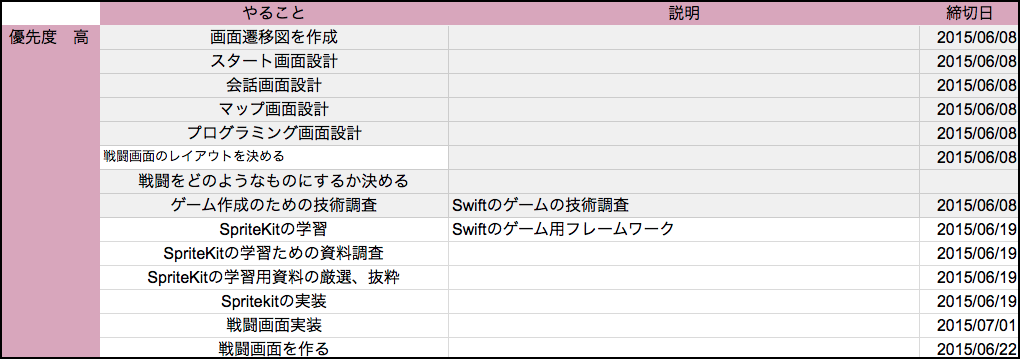
\includegraphics[width=14cm, bb=0 0 1020 359]{img/SprintBacklog.png}
\end{center}
\caption{6、7月分のバックログの原案}
\end{figure}

\begin{figure}[H]
\begin{center}
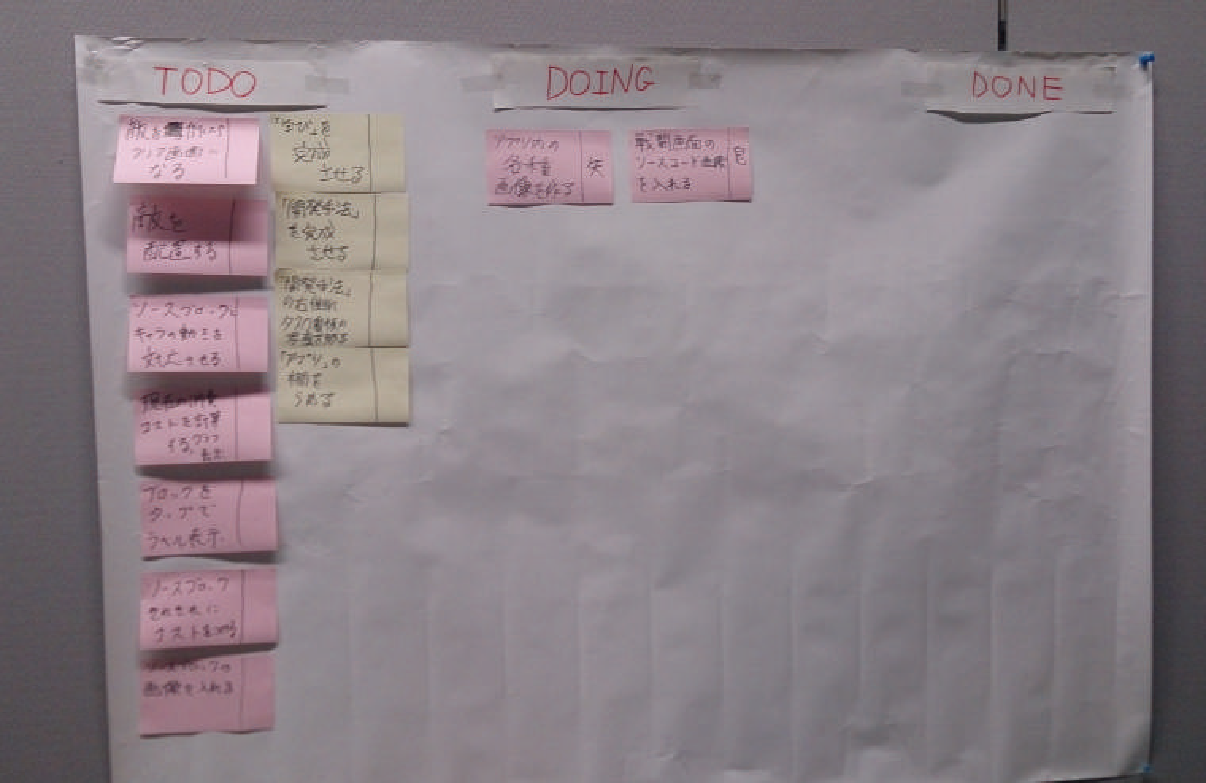
\includegraphics[width=14cm, bb=0 0 1206 783]{img/TaskKanban.png}
\end{center}
\caption{タスクかんばんのシステムを取り入れたバックログ}
\end{figure}

\bunseki{熊谷優斗}

\subsection{中間発表会の資料制作}
\par 中間発表会に向けて、ポスターを制作した。制作にあたって、グループメンバーを実装班3人とポスター班2人に分け、ポスターの制作が終わったら実装班がレビューをする、という形式をとった。しかし、メンバー間の意識共有が上手く行われていなかったため、実装班がポスターのレビューを上手く行うことが出来なかった。そのため、ポスターをTAや担当教員に見せたところ、目的と制作物がずれている、というレビューを受けた。これを受けて、メンバー5人全員で、一度背景、目的、課題の見直しを行い、ポスターの作り直しをした。しかし、短期間で急いでポスターの作り直しを行ったため、今度は文字が多すぎて見づらいというレビューを受けた。これを受けて、ポスター内の文字を少なくするため、もう一度ポスターの構成を見直すという作業を行った。結果、ポスターを作り上げることができたが、その制作に多くの時間を割くことになってしまった。ポスターやその他ドキュメントを作る際には、まずメンバー間の意識共有を行い、どういった構成で文書を書いていくか考えることに時間をかけるべきだ、ということを学んだ。

\bunseki{熊谷優斗}

\subsection{中間発表会}
\par 中間発表会ではメンバーを前半3人、後半2人に分けて、発表を行った。前半の発表では、アプリのデモを行わないと内容が伝わりづらい、というレビューを受けた。これを受けて後半の発表では、デモを取り入れ、内容が伝わりやすいようにした。しかし、後半の発表では合計で9人しか見に来た人がいなかった。このことから、教育系が開発しているアプリに魅力が少ないのではないか、という気づきを得た。

\bunseki{熊谷優斗}

\section{アプリ案の変化と内容}
\par プロジェクトを進めるうちに、アプリ内容、対象ユーザーが変化していった。その内容を以下に記す。
\bunseki{熊谷優斗}

\subsection{アプリ案の検討}
\par メンバーそれぞれが考えて来た案を評価し、5種類の案に絞った。図3.4に案を表す。

\par 5種類それぞれの案をメンバー内で肉付けした後、TAと担当教員からレビューを受けた。それぞれの案の詳細とレビューの内容を以下に示す。

\begin{description}
 \item[案1 いじめ対策アプリ]
従来相談を受けてもらうためには、電話をかけ、言葉で喋らなければならないので、ハードルが高い。一部の教育委員会では、メールの対応も行っている。そこで、少しでもハードルを下げるために、LINEのように教育委員会と会話ができるようにする。
	\begin{description}
 	\item[レビュー内容]
	このままだとただチャットをするだけのアプリになってしまうのではないか。既存のSNSアプリと差別化を行うため、独自の機能が必要である。また、どのようにしてこのアプリの評価を行うかという点は要検討である。
	 \end{description}
 
  \item[案2 プログラミングを学ぶゲームアプリ]
子供がゲーム攻略を楽しみながら、いつのまにかプログラミングを覚えることができるアプリである。最終的なユーザーの到達点としては制御文が使えるようになること。
	\begin{description}
 	\item[レビュー内容]
	ゲーム内容は、答えを導くのに手間がかかり、ユーザーに達成感があるものにすべきである。似たようなアプリは既にいくつも存在しているため、それらを調査し、どのように差別化を図るか検討する必要がある。
	 \end{description}

  \item[案3 発想力を鍛える−生産消費的なゲームアプリ]
  ユーザーが生産側と消費側の両面で機能することにより、全ユーザーで一緒に発想力を磨いていくアプリである。自分よがりの発想力ではなく、他人にも共感できる発想力を身につけさせることが目的。
	\begin{description}
 	\item[レビュー内容]
	ユーザー依存型アプリは投稿が増えないと開発が進まない可能性があるため、どうしたらユーザー同士で活発に活動してもらえるか考えるべきである。
	 \end{description}
	 
 \item[案4 1問1答共有アプリ]
  ユーザーが作った1問1答を共有するアプリである。問題を作る楽しさと問題を解く楽しさをシェアすることができる。
	\begin{description}
 	\item[レビュー内容]
	案3と同様に、どうしたらユーザー同士で活発に活動してもらえるか考える必要がある。投稿者が何か得をするシステムにしなければ問題の投稿数は増えていかないだろう。
	 \end{description}
	 
 \item[案5 外遊び支援アプリ]
遊びの教育を行う。IT化が進み、外で遊ぶことが少なくなってきている子供たちに対し、ITを活用することで供に外で遊んでもらう機会を増やす。その1つの案として、GPS機能を使って鬼ごっこを行う。
	\begin{description}
 	\item[レビュー内容]
	このアプリを開発するのであれば、楽しく開発を行えるだろう。しかし開発者が楽しくてもユーザーが楽しいとは限らない。ユーザーがどのような遊びを求めているか調査する必要があるだろう。また、アプリを使いながら鬼ごっこをすると、歩きスマホのような状態になり危険なのではないか。
	 \end{description}

 \end{description}
 
 \par レビューを受け、グループ内で検討した結果、前期では「案2 プログラミングを学ぶゲーム」を作成することに決定した。
 
 \begin{figure}[H]
\begin{center}
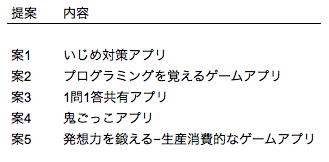
\includegraphics[width=12cm, bb=0 0 329 162]{img/AppIdea.png}
\end{center}
\caption{絞った5種類のアプリ案}
\end{figure}
 
 \bunseki{熊谷優斗}
 
 \subsection{大学生向けプログラミング入門アプリ}
\par 前述の「案2 プログラミングを学ぶゲーム」についてより深く考えていった結果、「既存の類似アプリと相違点を持たせるため、函館要素を追加しよう」、「子供は地域性に対してあまり興味を示さない、ならば対象ユーザーを未来大生にしよう」といった理由から、未来大学に入学することが決まった高校生に対するProcessing導入アプリを作成する方針が決まった。未来大1年生が「情報表現入門」でプログラミング言語「Processing」を学ぶ際につまづきやすいポイントを入学前に、ゲーム形式で気軽に学べることをアプリの目的とした。図3.5と図3.6はアプリ内画面のイメージ図の一部である。

\par 図3.6、通称「プログラミング画面」では、Scratchのように主人公の行動を表すブロックを組み立ててゆく。主人公はこのブロックの通りに動くので、どのようなブロックを組めば敵を倒すことができるかを考える必要がある。更に、「コスト」という概念を定義し、ブロックそれぞれをコストで重み付ける。1ターンで使用できるコストの上限は決まっているので、ユーザーはどのようにブロックを組めば同じコストでも最も多く行動できるかを考える必要がある。例えば、ループ文を使うことで、単純に同じブロックを何度も使用するよりも少ないコストで済む。これによりユーザーは自然と良いアルゴリズムを学ぶことができる。
\par このアプリ案をTA、担当教員、企業講師の方々に見せたところ、様々なレビューを受けた。一部を抜粋すると次のようなものである。
\begin{itemize}
 \item このアプリをプレイしたところで、本当にプログラミングの教育になるのだろうか。肝心のプログラミング画面の内容が薄く、未来大生がつまづきやすいポイントを学べるとは思えない。どうすればユーザーへの「教育」になるかを練り直すべき。
 \item 大学生が使うにしては、プログラミング画面の内容が低年齢向けである。
 \item もしアプリを一般向けにリリースすることを目標としているのであれば、未来大学入学向けアプリというのは対象ユーザーが狭すぎる。
 \end{itemize}
\par このレビューを受けて、もう一度メンバー内で教育要素について考え直し、対象ユーザーを全国の高校生、大学生向けへと変更した。また、プログラミング画面にて、「→」「パンチ」といった簡単な記述ではなく、「move(right, 3)」「attack(up)」といった、より本物のソースコードに近い形で表示するようにし、そのソースコードはボタンをタップしていくことで組み立てることができる仕組みにした。

\begin{figure}[H]
\begin{center}
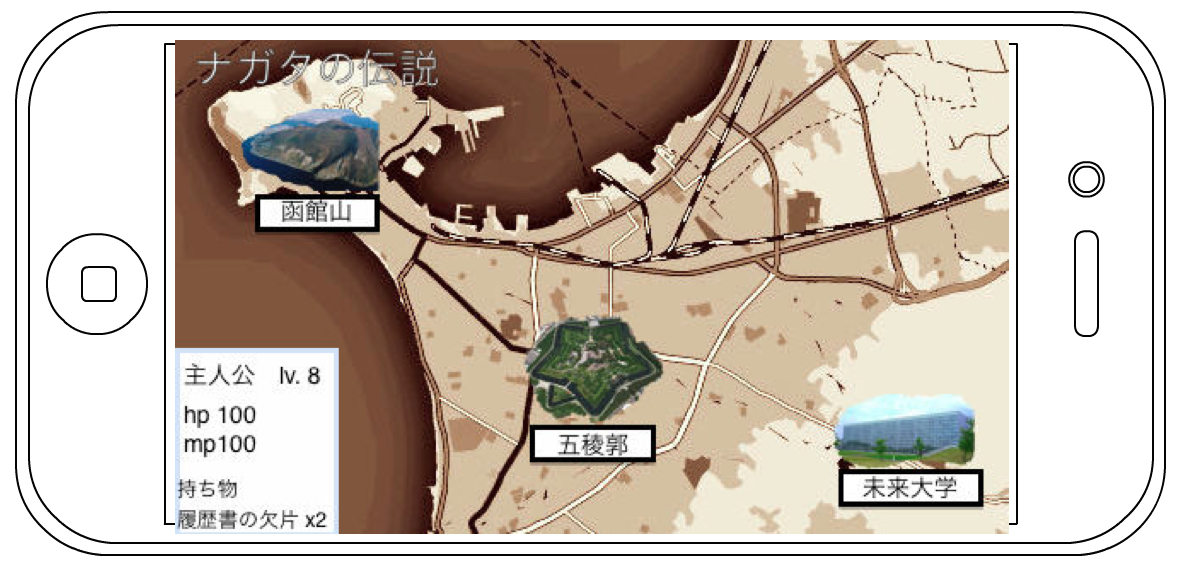
\includegraphics[width=12cm, bb=0 0 1182 571]{img/LengedOfN_map.png}
\end{center}
\caption{マップ画面}
\end{figure}

\begin{figure}[H]
\begin{center}
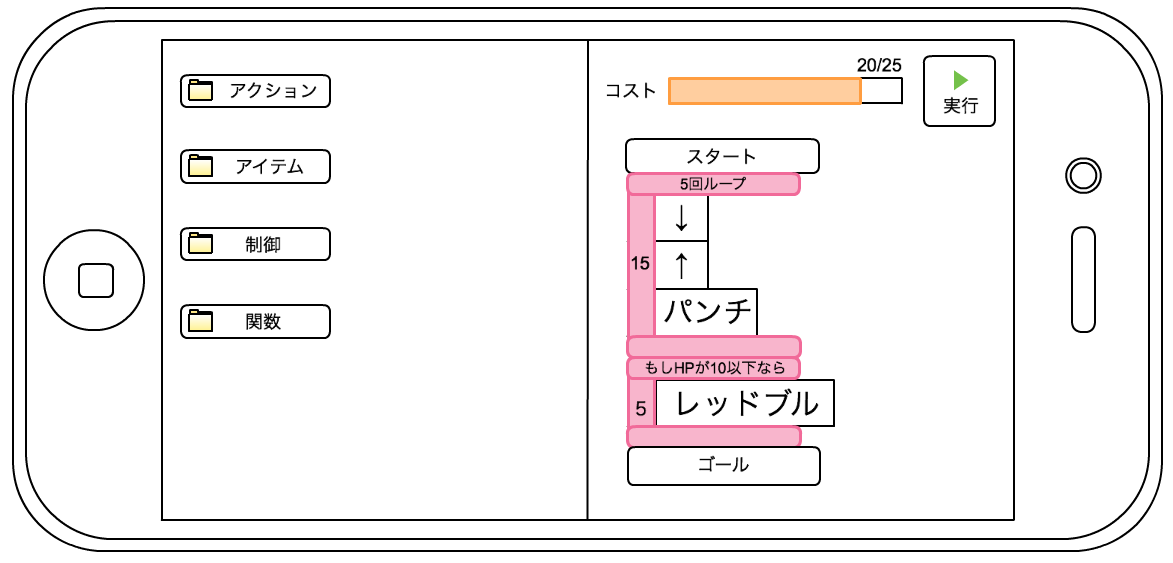
\includegraphics[width=12cm, bb=0 0 1173 563]{img/LegendOfN_programming.png}
\end{center}
\caption{プログラミング画面}
\end{figure}
 \bunseki{熊谷優斗}
 
 \subsection{中学生向けプログラミング支援アプリ}
\par プロジェクトを進めるうちに、大学生向けプログラミング入門アプリでは、プロジェクトとしての背景が、客観的に見て共感されないような内容であることに気がついた。そこで、日本の中学校ではプログラミング教育が義務化されている、また、現状のアプリ内容であれば、小学生、中学生が利用しても問題がないといった理由から、対象ユーザーを変更すべきであるという結論にたどり着いた。この日の議論により生まれたのが現状の背景(第1章にて記載)であり、現状のアプリ案(第4章にて記載)である。

\bunseki{熊谷優斗}


\chapter{開発アプリについて}
\section{概要}
開発するアプリは中学生でプログラミングを習った人、興味を持った人を対象としたプログラミングの組み方を学ぶゲームアプリである。
マス目上のステージにある自機をプログラムを組んで動かし、敵機を倒すことでゲームがクリアとなる。
\bunseki{新保遥平}

\subsection{ゲーム性}
ただプログラミングを学ぶのではなく、ゲームを通してプログラミングを学ぶことでユーザーのモチベーションを保ちつつ、アプリを使ってもらえるのではないかと考えた。また実際にプログラムを組むことで自機を思い通りに動かすことが出来たときにプログラミングの学習が深まるのではないかと考えた。
 
\bunseki{新保遥平}

\subsection{教育性}
このアプリではユーザーがプログラムの組み立て方を学ぶことを目的にしている。これを実現するために、このアプリにはコストとランクがある。ソースのボタンそれぞれにコストが設けられており、問題をクリアした際にコストの使用量が少ないほどよい簡潔にプログラムを組み立てることが出来たと判定し、ランクを与える。ランクが低かった場合、より良いランクにつながるヒントを与える。そして高いランクが与えられたときに、ユーザーを褒める言葉を表示する。このサイクルが次の問題への意欲につながる。またより簡潔なプログラムを組み立てることが出来るようになる。
\bunseki{新保遥平}

\section{プログラミング画面}

ユーザーは図4.1のように画面右側に配置されたそれぞれのソースボタンをタップして、プログラムを組んでいく。主なソースボタンはattack()、move()、left、right、0〜9などである。タップされたソースボタンは順に、右側のスペースに記述される。例えば下記のようにプログラムを組むことができる。
\par move(left,3);
\par move(up,3);




このようにプログラムをタップで組むことが出来る。また、間違ったタイミングでソースボタンを押すと画面上にエラーが出てすぐに確認ができる。

\begin{figure}[H]
\begin{center}
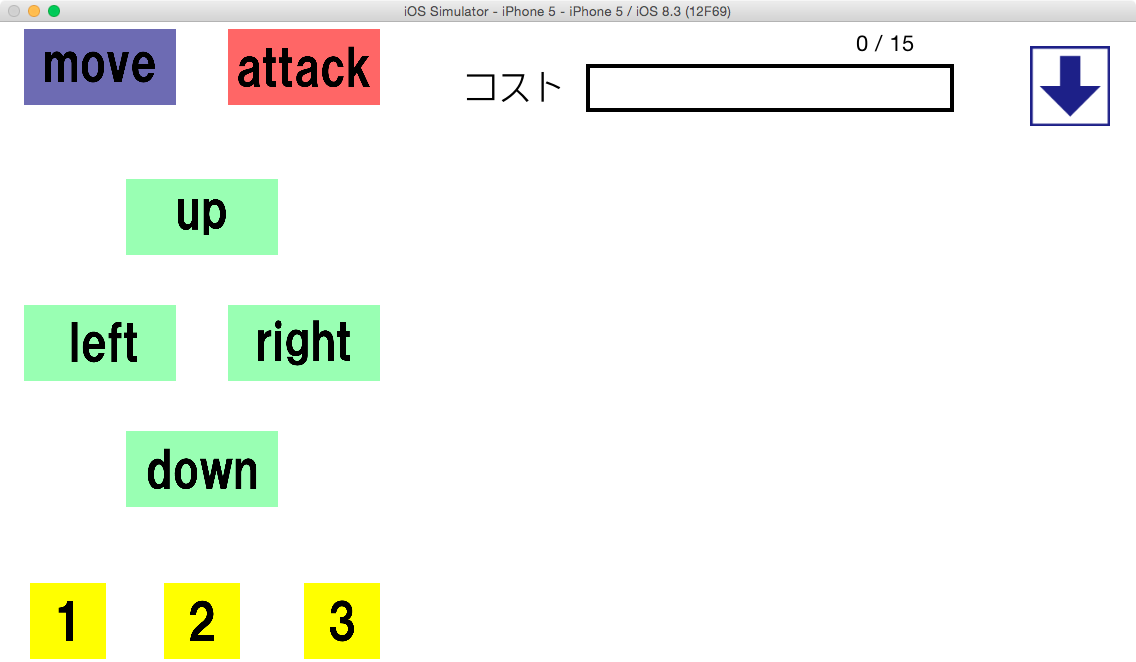
\includegraphics[width=10cm, bb=0 0 1136 662]{img/Prog-ra_programming.png}
\end{center}
\caption{プログラミング画面}
\end{figure}

\bunseki{新保遥平}

\section{戦闘画面}
図4.2の戦闘画面はプログラミング画面で入力したソースコードを実際に動かすための画面である。ソースコードを入力後、戦闘画面にある実行ボタンを押すことで、実機を動かすことが出来る。1回の実行で敵機を倒すことができるプログラムを組まなければならない。現状では、あらかじめ決められたプログラムでしか実機を動かすことが出来ない。

\begin{figure}[h]
\begin{center}
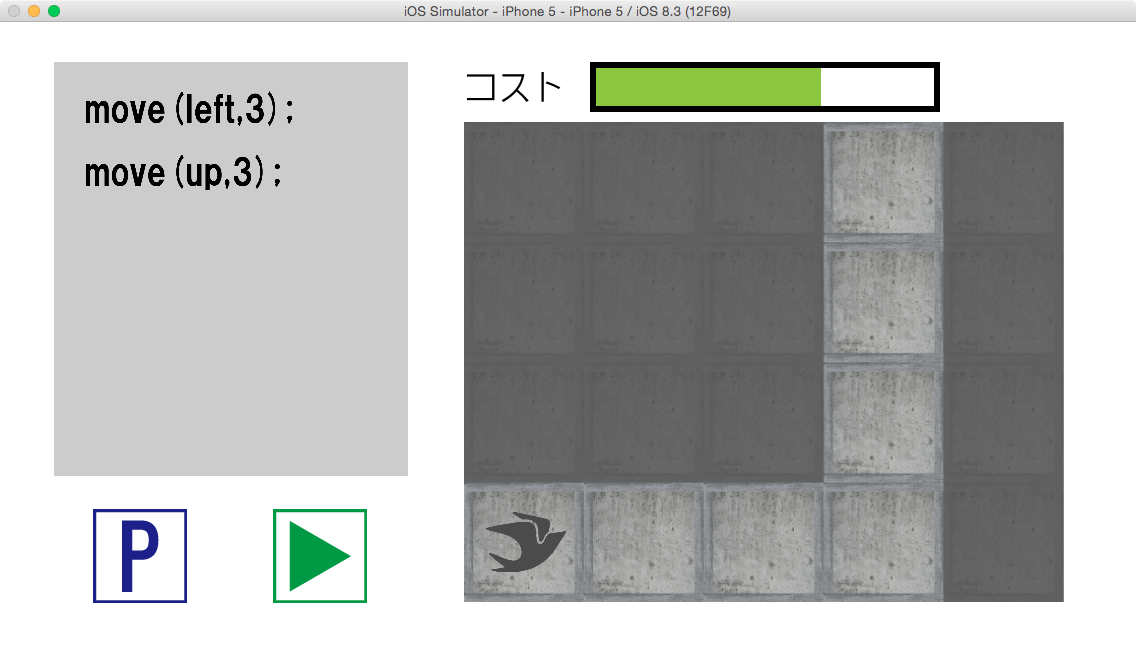
\includegraphics[width=10cm, bb=0 0 1136 662]{img/Prog-ra_Battle.png}
\end{center}
\caption{戦闘画面}
\end{figure}




\bunseki{新保遥平}

%5章
\chapter{結果}
\section{プロジェクトの評価}
7月に行われた中間発表会の評価シートの結果から、「声がはっきり聞こえた」、「声は大きく聞きやすかった」などの意見をいただき、発表技術に関しては高い評価を得られた。しかし、発表内容に関しては「最終的なゴールは?」、「まだ内容が決まっていないので評価不能」、「既存のもとの比較がない」などの意見をいただいた。これらの意見をまとめると、私たちのプロジェクトは目標が決まっていなく、内容がわかりづらいという評価であった。
\bunseki{中進吾}

\section{プロジェクトの成果}
小・中学生にプログラミングを教える場合、C言語やJavaから始めるのではなく、Scratchのようなビジュアルプログラミング言語から始めた方が良いということがわかった。また、プログラミングでラジコンやロボットを動かしてもらうことにより、プログラミングに興味を持ってもらうことができるということがわかった。
\bunseki{中進吾}


\chapter{まとめ}
\section{今後の課題と展望}
今後は、現在のアプリ案を再考し、より具体的で一貫性がある設計案にしていく必要がある。また、実際にゲームの内容を考えることや実証実験や評価方法を適切に定める必要がある。
\par
制御文のソースボタンやフィードバック機能を実装し、教育アプリとしての体裁を整え、11月に開催されるアカデミックリンクにてワークショップを開き、そこで得たレビューを活かしてアプリの改善を行うことが今後の展望である。
\bunseki{皀勢也}

\section{学び}
要件定義を固めずに実装を行ったため、プロジェクトの目的を見失い要件定義を一から考え直すことになった。そのため、時間をかけて、要件定義を行うことの重要性を学んだ。また、議事録を残していないことがあり、情報共有がうまくできていなかったことからドキュメントを残して、情報共有することの大切さを学んだ。
\bunseki{皀勢也}

% 以降、付録(付属資料)であることを示す
\begin{appendix}

\chapter{新規習得技術}
%\begin{hissu}
%課題解決過程に習得した技術について解説する。
%\end{hissu}

\chapter{活用した講義}
%\begin{hissu}
%課題解決過程において活用した講義について、講義名・活用内容を記述する。 
%\end{hissu}

\chapter{相互評価}
%\begin{hissu}
%課題解決過程で分担し、連携した作業全般について、互いに客観的に評価する。 
%\end{hissu}

\chapter{その他製作物}
%\begin{hissu}
%その他成果物をプロジェクトの担当教員の指示に従って添付する。
%\end{hissu}

%付録の終わり
\end{appendix}


%\backmatter

% 参考文献
\begin{thebibliography}{9}
% \bibitem {ラベル} 著者名. 書籍名. 出版社,  年号.
% \bibitem {A2} ほげほげお. うんたらかんたら,  2003.
\end{thebibliography}

\end{document}